\documentclass[twocolumn,a4paper,10pt]{ltjsarticle}

\usepackage{amsmath,amssymb}
\usepackage[T1]{fontenc}
\usepackage{mathptmx}
\usepackage[scaled=0.92]{helvet}
\usepackage{courier}
\usepackage{graphicx}
\usepackage{booktabs}
\usepackage{longtable}
\usepackage{enumitem}
\usepackage{caption}
\captionsetup{font=small,labelsep=quad,hypcap=false}
\usepackage[compact]{titlesec}
\usepackage{indentfirst}
\titlespacing*{\section}{0pt}{1.0ex plus .2ex minus .2ex}{0.5ex plus .1ex}
\titlespacing*{\subsection}{0pt}{0.6ex plus .2ex minus .1ex}{0.3ex plus .1ex}
\setlength{\parindent}{1em}
\usepackage{geometry}
\geometry{a4paper,left=15mm,right=15mm,top=18mm,bottom=18mm,
  headheight=16pt,headsep=4mm,includehead}
\setlength{\columnsep}{8mm}
\usepackage{fancyhdr}
\usepackage{hyperref}
\hypersetup{hidelinks}
\setlength{\textfloatsep}{4pt plus 1pt minus 1pt}
\setlength{\floatsep}{4pt plus 1pt minus 1pt}
\setlength{\intextsep}{4pt plus 1pt minus 1pt}
\setlength{\dbltextfloatsep}{6pt plus 1pt minus 1pt}
\setlength{\abovecaptionskip}{2pt}
\setlength{\belowcaptionskip}{0pt}
\setlength{\abovedisplayskip}{3pt plus 1pt minus 1pt}
\setlength{\belowdisplayskip}{3pt plus 1pt minus 1pt}

\newcommand{\venue}[1]{\def\thevenue{#1}}
\newcommand{\authornames}[1]{\def\theauthornames{#1}}
\newcommand{\affiliations}[1]{\def\theaffiliations{#1}}
\newcommand{\abstracttext}[1]{\def\theabstracttext{#1}}
\newcommand{\pdfmetaauthor}[1]{\def\thepdfauthor{#1}}
\newcommand{\contactinfo}[1]{\def\thecontactinfo{#1}}

% Place unnumbered contact information at the bottom of the first column.
\newcommand{\printcontactinfo}{%
  \begingroup
  \renewcommand{\thefootnote}{}%
  \footnotetext{\scriptsize \thecontactinfo}%
  \endgroup}

\makeatletter
\renewcommand{\maketitle}{%
  \hypersetup{pdftitle={\@title},pdfauthor={\thepdfauthor},pdfsubject={\thevenue}}%
  \twocolumn[{%
    \begin{center}
      {\LARGE\bfseries \@title\par}
      \vspace{8pt}
      {\large \theauthornames\par}
      \vspace{4pt}{\normalsize \theaffiliations\par}
      \vspace{9pt}
    \end{center}
    \begin{center}
      \begin{minipage}{0.86\textwidth}
        \begin{center}\textbf{Abstract}\end{center}
        \vspace{1pt}\theabstracttext\par
      \end{minipage}
    \end{center}
    \vspace{10pt}
  }]%
}
\makeatother

\let\oldthebibliography\thebibliography
\renewcommand{\thebibliography}[1]{%
  \setlength{\topsep}{0pt}%
  \oldthebibliography{#1}\footnotesize
  \setlength{\itemsep}{1pt}\setlength{\parsep}{0pt}}

\fancypagestyle{firstpage}{%
  \fancyhf{}
  \renewcommand{\headrulewidth}{0.4pt}
  \fancyhead[C]{\large \thevenue}}
\AtBeginEnvironment{thebibliography}{\footnotesize}
\pagestyle{empty}

\venue{言語獲得と理解研究会報告（Summer 2026）}
\title{日本語省略質問に対する検索・クエリ拡張手法の体系的評価}
\authornames{%
  井原 惇宏\textsuperscript{1}\quad
  ジェプカ ラファウ\textsuperscript{2}}
\affiliations{%
  \textsuperscript{1}\,北海道大学大学院情報科学院\quad
  \textsuperscript{2}\,北海道大学大学院情報科学研究院}
\contactinfo{〒060--0814 北海道札幌市北区北14条西9丁目\\
  E-mail: \texttt{atsu.1129.mt@gmail.com}}
\pdfmetaauthor{Atsuhiro Ihara, Rafal Rzepka}
\abstracttext{%
We investigate how information omission affects Japanese document retrieval and how retrieval and query expansion methods respond to it.
From 306 candidates based on JDocQA, human evaluation retained 276 queries covering three grammatical cases and four semantic categories.
We compare seven methods on retrieval of the original evidence page from a collection of 510 pages, using document-grouped validation.
Omission reduced mean reciprocal rank (MRR) across all five methods evaluated on both original and omission queries.
Weighted sparse--dense fusion achieved the highest MRR of 0.8460 on omission queries, compared with 0.8333 for BM25, although the difference was not statistically significant.
For Query2doc-style expansion, increasing the weight of the remaining query terms from one to five raised MRR from 0.8158 to 0.8423 with BM25 parameters and generated text held fixed.
Selecting retrieval methods by gold omission category did not outperform selecting a single method across categories.
These results highlight the importance of preserving the contribution of remaining query terms in expansion and show that omission categories alone did not yield better method selection.}
\begin{document}
\maketitle
\thispagestyle{firstpage}
\printcontactinfo
\section{はじめに}
検索拡張生成（Retrieval-Augmented Generation; RAG）\cite{lewis2020rag}では，質問に関連する文書を検索し，生成モデルへ与える．
質問から対象を特定する情報が省略されると，正解根拠への到達が難しくなる可能性がある．佐々木・山本はJDocQAを用い，省略が密検索性能を低下させることを示した\cite{sasaki2026ambiguity}．
一方，既存の検索・拡張手法がどの条件で省略の影響を緩和するかは十分に明らかでない．

本稿で扱う「曖昧クエリ」は，JDocQAの正解回答と根拠ページが付与された質問から，格や意味役割のカテゴリに基づいて情報の一部を省略したクエリであり，以降「省略質問」と呼ぶ．省略後も残る情報だけで検索対象を特定できる場合と，特定が難しくなる場合がある．本稿では，元質問の根拠ページを検索できるかを評価する．
JDocQA~\cite{onami2024jdocqa}に基づく7カテゴリ・276件の省略質問で，クエリ拡張を組み合わせた方式も含む7種類の検索手法を比較し，以下を検証する．
(RQ1) 省略による検索性能の低下は検索手法間でどう異なるか，(RQ2) どの検索手法が高い性能を示し，その利点は省略に特有か，
(RQ3) 省略カテゴリ別の検索手法選択は全カテゴリ共通の検索手法選択を上回るか．

本稿の貢献は，(1) 格と意味役割の二つの観点から，7カテゴリの人手評価済み省略質問データセットを構築すること，
(2) 省略質問に対する7種類の検索手法の性能を比較すること，
(3) 省略カテゴリ別の検索手法選択の限界を検証・考察することである．
\section{関連研究}

佐々木・山本は，日本語RAG検索における省略由来の曖昧クエリを対象とし，省略が
密検索のRecallを低下させることに加え，検索スコアの分散と上位文書の意味的一貫性が
曖昧性検知の手掛かりになることを示した\cite{sasaki2026ambiguity}．同研究は，日本語の
文書質問応答データセットJDocQA~\cite{onami2024jdocqa}から106質問を抽出し，質問から
主語・目的語・修飾語等を省略した条件を検証している．これは省略質問を検索時点で検知し，
不足情報の確認や補完へ接続する重要な問題設定である．一方，同研究の検索実験は密検索を
中心としており，省略の種類と，異なる検索・改善手法との関係には体系的比較の余地が残る．

日本語では，文脈から回復可能な述語の項が明示されない項省略が広く生じる．Ishizukiらは
日本語均衡コーパスから2,000件を超える項省略判断を収集し，省略可否とその言語的要因を
分析した\cite{ishizuki2024drop}．また，日本語の述語項構造・ゼロ照応解析では，省略された
項をガ格（主格），ヲ格（対格），ニ格（与格）に分けて同定・解析する枠組みが用いられている
\cite{sasano2011zero}．これらは省略を述語に対する項の関係から捉える知見である．これに対し，
検索への影響は，省略された情報が人物・組織，場所・管轄，時間，対象・内容・属性のいずれか
という意味内容によっても異なり得る．本研究では，前者の格に基づく3分類と，後者の意味内容に
基づき操作的に定めた4分類を同一の分類体系とはみなさず，二つの観点から省略の影響を分析する．

情報検索には，語彙的一致を利用する疎検索と，質問・文書の意味表現を用いる密検索がある．
本研究では，疎検索の代表としてBM25~\cite{robertson2009bm25}，密検索の代表として密ベクトル
検索\cite{karpukhin2020dpr}を扱う．両者は省略後に残る検索信号が異なるため，省略に対する
頑健性も異なる可能性がある．さらに，両検索器の相補性を利用する方法として，順位を統合する
Reciprocal Rank Fusion（RRF）\cite{cormack2009rrf}と，正規化スコアの線形統合を比較する．

不足した検索信号を補う別の方法がクエリ拡張である．疑似適合フィードバックは初回検索の
上位文書から適合モデル\cite{lavrenko2001relevance}を推定し，RM3はこれを元クエリと補間して
再検索する\cite{jaleel2004rm3}．Query2docは，大規模言語モデルが生成した疑似文書を元クエリへ
連結する\cite{wang2023query2doc}．原研究ではMS MARCO~\cite{nguyen2016msmarco}，
TREC Deep Learning Track~\cite{craswell2020trec}，BEIR~\cite{thakur2021beir}等で改善が
報告されている．一方，省略質問では不足した具体的実体を一意に復元できるとは限らず，初回検索や
生成内容が誤れば，追加語が検索意図を変えるクエリドリフトを生じ得る．

以上を踏まえ，本研究は佐々木・山本の問題設定を継承し，省略質問に対して7種類の
検索・改善手法を共通のデータ・分割・評価指標で比較し，正解カテゴリを追加入力する方式は区別する．さらに，二つの観点から定めた7カテゴリについて性能差と
失敗要因を調べ，省略カテゴリだけで有効手法を選択できるかを検証する．本研究の目的は，新規検索器を
提案することではなく，既存手法が日本語省略質問へ移転する条件と限界を明らかにすることである．
この分析は，将来的に質問文だけでなく検索スコア，検索器間の不一致，上位文書の一貫性等を用いて
検索失敗を検知し，必要な場合だけ補完や確認質問へ接続する選択的な検索処理の基礎となる．

\section{データセット構築}

\subsection{元データと省略生成}

本研究では，検索評価用データセットの元質問と検索対象文書をJDocQAから構築した．構築した省略質問データセットをGitHubで公開している\footnote{\url{https://github.com/Language-Media-Lab/Japanese-omission-query-retrieval}}．
JDocQA収録質問のうち，回答が文章で記述され，回答不能理由がなく，画像のみを根拠としない
510質問を候補母集団とした．このうち，先行研究と共通するvalidation/test split由来の
106件を基本集合とし，格省略の候補を確保するためにtrain split由来の404質問を追加した．
元質問と正解回答は変更せず，質問末尾の定型的な回答指示
「解答は自由に記述してください。」のみを除去した．

格省略は，日本語統合解析器KWJA~\cite{ueda2023kwja}（2.5.1，baseモデル，rhoknp 1.8.0）の述語項構造解析を用いて，明示された
ガ格・ヲ格・ニ格の項を文字列上から機械的に削除した．解析格と表層助詞が一致し，項が述語へ
直接係り，項に修飾句が付かず，削除位置を一意に復元できる候補だけから各格40件，計120件を選んだ．ニ格，ガ格，ヲ格の順に，seed 20260716と候補IDのハッシュ値による決定的な順序で抽出し，格省略120件内で元質問の重複を避けた．意味役割による省略は，人物・組織，
場所・管轄，時間，対象・内容・属性の4カテゴリとした．固定106質問に対し，gpt-5-miniと
カテゴリ定義を含む意味役割4カテゴリ生成プロンプト（\ref{app:prompt}）で候補を生成した．モデルには元質問，PDF
メタデータ，正解回答，根拠本文の先頭3,000文字を与え，出力は元質問中の明示表現の削除と最小限の
文法修正に限定するよう指示した．この指示への出力の適合を保証するものではなく，追加監査で規則から外れる編集も確認された（\ref{app:agreement}）．最大出力は6,000 token（temperature・seed未指定）である．カテゴリは元質問内の
意味役割で排他的に付与し，回答・根拠からの情報追加は禁止した．人物・組織39件，時間46件，場所51件は生成候補を全件使用し，対象・内容・属性はseed 20260716とカテゴリ・質問ID・省略後質問のハッシュ値による順序で50件を抽出した．意味役割省略は計186件である．各カテゴリの定義と実例は\ref{app:examples}に示す．

\subsection{人手評価と選別}

格省略120件と意味役割省略186件の計306質問を4バッチへ分け，クラウドワークス\footnote{\raggedright クラウドソーシングサービス「クラウドワークス」：\url{https://crowdworks.jp/}\par}で募集した14名が評価した．主評価の12名は
1人76--77件を担当し，各質問を独立した3名が評価した．固定報酬は1人当たり税抜3,000円，想定作業時間は
約2時間とした．生成AI・自動評価ツールの使用と評価者間の相談を禁止し，未入力，不正値，固定列の改変，
不自然な一律回答の有無を確認した．自然性は1（自然），2（やや不自然），3（不自然），回答可能性は1（回答可能），2（条件付きで回答可能），3（回答困難）の3段階とした．回答可能性の2は，正解回答が候補になるが見出し・周辺文脈・対象の補足が必要な場合である．
評価者には元質問，省略後質問，省略情報，正解回答を提示し，回答可能性では「適切な文書がすでに特定され，参照できる」と仮定した．これは検索可能性や，質問単独での意図の一意性を測る評点ではない．
意味役割4カテゴリではカテゴリ名を提示し，妥当性を1（妥当），2（判断が分かれる），3（不適切）で評価した．元の3名で評価1と3が混在した76質問には，
残る2名によるブラインド評価を追加した．通常項目は3名，追加対象は5名の中央値を合意値とした．
自然性または回答可能性の中央値が3の30件を除外し，276件を検索実験に用いた．
カテゴリ妥当性は選別条件には使用せず，カテゴリ別解析時の注意情報として保持した．評価対象186件中，その中央値が3の3件中1件は上記基準で除外され，2件（EVAL-0053, EVAL-0256）は276件に含まれる．公開先と本稿の訂正実験の対応は\ref{app:repro}に示す．この2件を含むカテゴリラベルの不確実性は，カテゴリ別分析の限界として扱う．

\begin{table}[tb]
  \centering
  \caption{評価用省略質問のカテゴリ別件数．}
  \label{tab:data}
  \begin{tabular}{lrr}
    \toprule
    分類 & カテゴリ & 件数 \\
    \midrule
    格解析 & ガ格 & 36 \\
           & ヲ格 & 32 \\
           & ニ格 & 32 \\
    \midrule
    意味役割 & 人物・組織 & 38 \\
             & 場所・管轄 & 49 \\
             & 時間 & 42 \\
             & 対象・内容・属性 & 47 \\
    \midrule
    \multicolumn{2}{l}{合計} & 276 \\
    \bottomrule
  \end{tabular}
\end{table}

表\ref{tab:data}に最終件数を示す．276省略質問は176元質問から生成され，176個の根拠文書を共有する．同じ元質問から複数の省略質問を作るためであり，検索コーパスの文書重複とは異なる．この依存を
無視したクエリ単位分割は，類似内容が開発・評価の双方へ入る漏洩を生じ得るため，以降の重み選択と
ルーティングでは根拠文書単位の5-fold分割を用いる．


\subsection{評価者間一致度}
順序尺度のKrippendorffの$\alpha$~\cite{hayes2007alpha}を，評点の周辺度数に基づく順序距離と，項目ごとの評価人数を考慮した一致行列から求めた．
表\ref{tab:agreement}は初回3名の全候補に対する結果である．
自然性と回答可能性の一致は十分に高いとはいえず，評価基準の解釈差が残る．カテゴリ妥当性のペア一致率は83.2\%だが，評点1が503/558評価（90.1\%）に集中し，偶然一致を補正する$\alpha$は0.1048にとどまる．
したがって，中央値3の項目が少ないことは，高い評価者間一致を意味しない．また，評点1・2・3の三者分裂でも中央値は2となり，多数決とは異なる．
\begin{table}[tb]
\centering\small
\caption{初回3名の一致度．一致率は同一質問内の評価者ペアが同じ評点を付けた割合（\%）．}\label{tab:agreement}
\begin{tabular}{lrrr}
\toprule
評価軸 & 質問数 & $\alpha$ & 一致率 \\
\midrule
自然性 & 306 & 0.5116 & 68.5 \\
回答可能性 & 306 & 0.3793 & 55.0 \\
カテゴリ妥当性 & 186 & 0.1048 & 83.2 \\
\bottomrule
\end{tabular}
\end{table}
追加対象では自然性・回答可能性が76件，カテゴリ妥当性が44件である．同じ追加対象で初回3名と5名を比較した$\alpha$は，
自然性0.1089から0.2189，回答可能性$-0.0748$から0.0732，カテゴリ妥当性$-0.0454$から0.0970となった．
初回の強い不一致に基づく選択集合であり，全候補とは分布が異なる．評価者構成も変わるため，この差を評価者自身の一致が改善した因果効果とは解釈しない．
生成方式別の値は\ref{app:agreement}に示す．
\section{検索手法と評価設定}
\subsection{文書・評価指標・分割}
JDocQAの根拠ページ1ページを1文書とし，510文書を検索対象とする．省略前の質問に付与された正解ページを，省略後の質問でも検索できるかを評価する．検索対象には，同じページや本文が完全に一致する文書の重複はない．

主指標をMean Reciprocal Rank（MRR），補助指標をRecall@$k$（以下R@$k$；$k=1,3,5,10$）とする．MRRは全510文書中の正解順位の逆数を276省略質問で等重み平均する．1正解条件でのR@$k$は，正解文書が上位$k$件に含まれる質問の割合である．一つの元質問から複数の省略質問を作成しているため，元質問ごとに平均してから全体を平均する補助集計も行った（\ref{app:sensitivity}）．
同じ根拠文書に対応する質問が調整用と評価用の両方に入らないよう，根拠文書単位でデータを5分割した．各分割を順に評価用とし，残りの4分割をパラメータの調整用に用いる．
同点スコアは文書ID順で解決する．元質問用の疑似文書は生成していないため，省略前後比較は密検索，BM25，RM3型，RRF，重み付き疎密統合の5手法に限定する．

\subsection{検索・拡張手法}
密検索はtext-embedding-3-small（1,536次元）の埋め込みをL2正規化し，内積で順位付けする．
BM25はNFKC正規化（全角・半角等の互換文字を統一），小文字化，空白除去後の文字bigramを用いる．外部形態素辞書に依存せず，同一規則を日本語・英数字へ適用するためである．
本稿の主比較では，質問中のbigramの出現回数$c_q(t)$を線形重みとして各語のBM25寄与に掛ける．質問語頻度の扱いをBM25単独，疎密統合，RRF，RM3型の初回検索で揃える．

RM3型は初回検索上位10文書から適合モデル\cite{lavrenko2001relevance,jaleel2004rm3}を推定し，選んだ上位bigram分布と質問の語頻度分布を補間して重み付きBM25で再検索する．
文書の重み推定にDirichlet平滑化（$\mu=1000$）を用いる．標準的な単語単位のクエリ尤度検索によるRM3の厳密な再現ではない．

Query2doc型は，省略質問からgpt-5-miniと日本語の4例を用いたプロンプト（4-shot）で疑似文書を生成し，検索語を拡張する．通常版は省略質問のみを入力し，カテゴリ条件付き版は正解の省略カテゴリ名と定義も与える．各検索条件で同じ保存済み生成文を用いた．プロンプトと生成条件の詳細は\ref{app:q2d}に示す．

元の質問語が生成文に埋もれないよう，原研究\cite{wang2023query2doc}にならって質問語の重みを5倍にする．本実装は質問と疑似文書を別々にbigram化し，
\begin{equation}
w(t)=n c_q(t)+c_p(t),\qquad n=5
\label{eq:qweight}
\end{equation}
をBM25の質問語重みとする．$c_p(t)$は疑似文書中の語頻度である．反復境界や\texttt{[SEP]}に由来する人工的なbigramを避けるため，文字列の反復連結ではなく頻度を加算する．$n=1$を補助条件とする．

RRFは密検索とBM25の順位を$1/(k+r)$の和で統合する．重み付き疎密統合は各質問について両検索器の全文書スコアを最小最大正規化し，
\begin{equation}
s(d)=\alpha s_{\mathrm{dense}}(d)+(1-\alpha)s_{\mathrm{BM25}}(d)
\end{equation}
で統合する．以降，本文・図表とも「密検索」「重み付き疎密統合」の表記を用いる．

\subsection{パラメータ選択と統計比較}
検索性能は，BM25の設定値や疎密統合の混合比率などによって変わる．そこで，特定の固定値だけに比較結果が依存しないよう，主比較では各検索手法のパラメータを調整してから評価する．密検索は固定した埋め込みモデルを用いる．
各回の調整用4分割で省略質問のMRRが最も高い設定を選び，その設定を評価用の1分割に適用する．評価用の正解情報は設定の選択に用いない．これを5回繰り返して，全質問の評価結果を集計する．省略前後の比較では，元質問にも省略質問と同じ設定を用いる．質問語の重み付けの影響を調べる補助比較では，他のパラメータと生成文を固定する．探索する値と候補数は\ref{app:parameters}に示す．

検索手法間の差は，同じ質問に対する結果を対応付けて検定する．同じ根拠文書から作られた質問の依存を考慮し，根拠文書単位で検定と95\%信頼区間の推定を行う．主比較では各検索手法とBM25のMRR差を調べ，複数の比較による偶然の有意差を抑えるためHolm補正を用いる．また，BM25に対する利得を省略前後で比較し，その利得が省略時に大きくなるかを調べる．統計処理の詳細も\ref{app:parameters}に示す．
\section{結果}
\subsection{省略前後の性能と頑健性}
表\ref{tab:beforeafter}に同じ開発側選択値を用いた省略前後の比較を示す．密検索のMRRは0.7702から0.7056，BM25は0.8734から0.8333へ低下した．
R@1はそれぞれ72.1\%から65.6\%，85.5\%から80.8\%である．重み付き疎密統合は元質問でもBM25を上回るため，省略質問での高性能だけから省略特有の頑健性とはいえない．
疎密統合のBM25に対するMRR利得は元質問0.0144，省略質問0.0127で，利得差は$-0.0017$（95\% CI [$-0.0206$, 0.0168]，未補正$p=0.8617$，Holm補正$p=1.0000$）であった．
省略時に利点が増す証拠は得られなかった．低下幅は元の性能水準にも依存するため，小さい低下幅だけで手法の優劣を判断しない．
\begin{table}[tb]
\centering\small
\caption{調整済み条件における元質問・省略質問のMRR．差は省略後から元を引いた値．}\label{tab:beforeafter}
\begin{tabular}{lrrr}
\toprule
手法 & 元質問 & 省略質問 & 差 \\
\midrule
密検索 & 0.7702 & 0.7056 & -0.0646 \\
BM25 & 0.8734 & 0.8333 & -0.0401 \\
RM3型 & 0.8721 & 0.8200 & -0.0521 \\
RRF & 0.8446 & 0.8073 & -0.0373 \\
重み付き疎密統合 & 0.8878 & 0.8460 & -0.0418 \\
\bottomrule
\end{tabular}
\end{table}
図\ref{fig:omission}はカテゴリ別R@1の差を示す．各カテゴリは32--49件であり，同じ根拠文書を共有する質問も含む．誤差範囲も踏まえ，カテゴリ差は探索的な記述にとどめる．
\begin{figure*}[tb]\centering
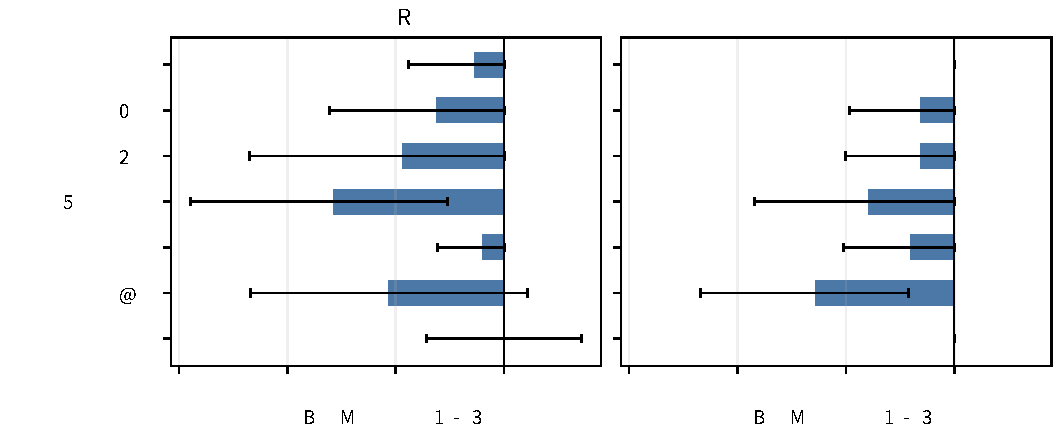
\includegraphics[width=\textwidth]{figures/review_20260911/omission_delta.pdf}
\caption{調整済み条件でのカテゴリ別R@1差（省略後$-$元）．誤差棒は根拠文書単位の95\%クラスタ・ブートストラップ区間であり，多重比較調整はしていない．}
\label{fig:omission}\end{figure*}

\subsection{検索改善手法の比較}
表\ref{tab:methods}は主比較である．密検索は固定モデル，その他は各foldの開発側で設定を選択した評価側結果を集約する．
重み付き疎密統合がMRR 0.8460で最も高いが，BM25との差$+0.0127$は有意でなかった（未補正$p=0.1267$，Holm補正$p=0.4006$）．R@1の最高値はカテゴリ条件付きQuery2doc型の81.9\%であり，疎密統合が全指標で最良ではない．
通常・カテゴリ条件付きQuery2doc型のMRRは0.8382，0.8447で，BM25より平均値は高いがHolm補正後$p$は0.4338，0.4006であった．RM3型とRRFも調整済みBM25に対する有意な改善を示さなかった．
\begin{table*}[tb]
\centering\small
\caption{省略質問の主比較．MRRは0--1，R@$k$は\%．太字は列内最高値．密検索以外は同じ外側5-foldの開発側でパラメータを選択した（探索候補数は本文参照）．}\label{tab:methods}
\begin{tabular}{lrrrrr}
\toprule
手法 & MRR & R@1 & R@3 & R@5 & R@10 \\
\midrule
密検索 & 0.7056 & 65.6 & 73.2 & 75.7 & 80.1 \\
BM25 & 0.8333 & 80.8 & 84.1 & 86.2 & 88.4 \\
RM3型 & 0.8200 & 79.3 & 83.0 & 84.4 & 87.7 \\
Query2doc型 & 0.8382 & 81.2 & 84.8 & 86.6 & 88.8 \\
Query2doc型（正解カテゴリあり） & 0.8447 & \textbf{81.9} & 85.1 & 87.3 & \textbf{90.2} \\
RRF & 0.8073 & 75.4 & 84.1 & 87.7 & \textbf{90.2} \\
重み付き疎密統合 & \textbf{0.8460} & 81.2 & \textbf{86.2} & \textbf{88.0} & \textbf{90.2} \\
\bottomrule
\end{tabular}
\end{table*}
\subsection{質問語の重み付けと拡張}
表\ref{tab:repeat}ではBM25の$k_1,b$と疑似文書を固定し，式\ref{eq:qweight}の$n$だけを変えた．通常版は$n=1$のMRR 0.8158から$n=5$の0.8423へ上昇した．
固定BM25（0.8278）との比較では$n=5$の通常版・カテゴリ条件付き版のHolm補正後$p$は0.0411，0.0461であった．ただし調整済み主比較の有意差は確認されず，固定条件での利得を一般化しない．
\begin{table}[tb]
\centering\small
\caption{固定BM25条件での質問語重みの比較．同じ生成方式の重み1・5間でキャッシュを共有し，条件付き版は正解カテゴリを利用する．}\label{tab:repeat}
\begin{tabular}{lrr}
\toprule
条件 & MRR & R@1 (\%) \\
\midrule
BM25 & 0.8278 & 80.1 \\
通常版，重み1 & 0.8158 & 78.3 \\
通常版，重み5 & 0.8423 & 81.9 \\
条件付き版，重み1 & 0.8122 & 77.5 \\
条件付き版，重み5 & 0.8388 & 81.2 \\
\bottomrule
\end{tabular}
\end{table}
初稿では質問を文字列として5回反復したが，検索処理で同一bigramを重複除去していたため，反復による重み増加が働いていなかった．
査読後の実装確認でこれを修正し，比較先BM25にも質問語頻度を適用して全手法を再評価した．旧方式の通常版MRR 0.7522に対し，旧結合形式を維持して語頻度だけを反映した値は0.8424で，現在の0.8423に近い．
したがって初稿の大幅悪化をQuery2docの枠組みやプロンプト制約だけに帰属できない．この比較も本研究の日本語プロンプトと文字bigram実装に限定される．

\subsection{クエリ単位のエラー分析}
図\ref{fig:transitions}に主比較における正解順位の変化を示す．調整済みBM25に対し，重み付き疎密統合は42件を改善し9件を悪化させた．
通常Query2doc型は25件・22件，カテゴリ条件付き版は29件・21件であった．Top-1だけを見るとRM3型は回復2件・悪化6件，通常版は4件・3件，カテゴリ条件付き版は6件・3件である．
これら拡張3方式の少なくとも一つが該当する質問を重複除去すると，回復7件・悪化8件となる．初稿の8件・32件は修正後条件には当てはまらない．
\begin{figure*}[tb]\centering
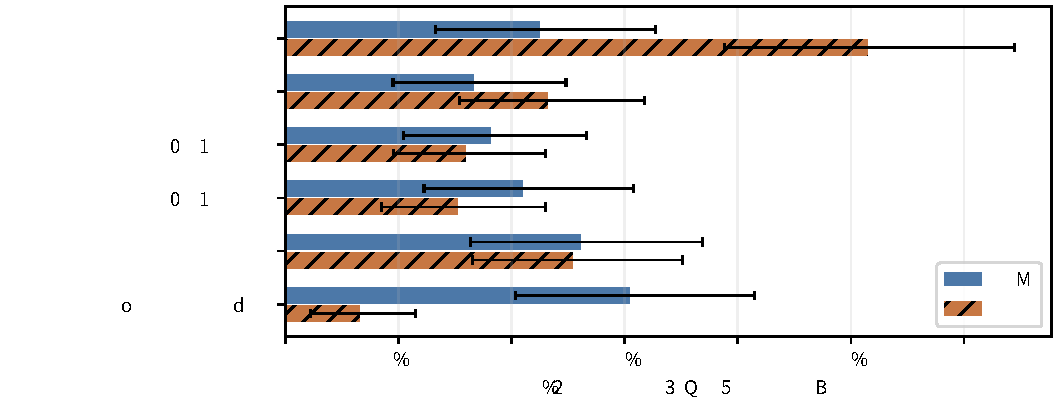
\includegraphics[width=\textwidth]{figures/review_20260911/rank_transitions.pdf}
\caption{調整済みBM25に対する正解順位の改善・悪化率．順位不変は省略した．カテゴリ条件付きQuery2doc型は正解カテゴリを利用する．誤差棒は根拠文書単位の95\%クラスタ・ブートストラップ区間（多重比較未調整）．}
\label{fig:transitions}\end{figure*}
順位変化だけから，誤った具体化，一般語の追加，質問語の相対的寄与の低下などの原因を特定することはできない．
追加語により検索意図がずれる現象をクエリドリフトと呼ぶが，修正後の全失敗を語彙的ドリフトと断定することは避ける．

\subsection{カテゴリ別ルーティング}
候補はBM25，RM3型，Query2doc型2方式，重み付き疎密統合の5手法とする．外側評価foldを完全に除いた開発集合で，根拠文書単位の内側4-foldを作成した（seedは20260911に外側foldの0始まり番号を加算）．
内側開発側だけで各手法のパラメータを選び，内側評価側の予測を集約したMRRから，全体で一つの手法，またはカテゴリごとの手法を選ぶ．
その後，選択手法のパラメータを外側開発集合で選び直し，外側評価集合へ適用した．従って表\ref{tab:methods}の特定手法の行と，表\ref{tab:routing}の単一手法選択の行が一致する必要はない．
カテゴリは正解ラベルを用いる分析条件であり，カテゴリ推定の誤りは含まない．候補集合にも正解カテゴリを入力する拡張方式が含まれる．

カテゴリ別選択はMRR 0.8387で，単一手法選択0.8422を上回らなかった（差$-0.0034$，95\% CI [$-0.0150$, 0.0072]，$p=0.5607$）．
5候補から評価質問ごとに事後的に最良を選ぶOracleは0.8703であった．Oracleは候補集合に依存し，手法追加で非減少となる非実用的上限である．この記述的な差だけで改善可能性を保証しない．
\begin{table*}[tb]
\centering\small
\caption{外側5-fold・内側4-foldによるルーティング．カテゴリ別選択は正解カテゴリ既知．候補5手法は正解カテゴリありの拡張を含む．Oracleは実運用性能ではない．}\label{tab:routing}
\begin{tabular}{lrrrrr}
\toprule
方式 & MRR & R@1 & R@3 & R@5 & R@10 \\
\midrule
単一手法選択 & 0.8422 & 81.2 & 85.1 & 87.3 & 90.2 \\
カテゴリ別選択（正解カテゴリあり） & 0.8387 & 81.2 & 85.1 & 85.5 & 89.5 \\
質問単位Oracle & 0.8703 & 84.4 & 88.8 & 89.9 & 90.9 \\
\bottomrule
\end{tabular}
\end{table*}
\section{考察と限界}
本データでは重み付き疎密統合が主指標の平均MRRで最高となったが，調整済みBM25に対する有意差も，省略時に特有の利得も確認されなかった．
したがって，有望な比較候補としての位置付けと，省略に頑健な手法であるという確証を区別する必要がある．
パラメータ選択の機会を与えても，有限の開発データによる選択は評価性能の上昇を保証しない．探索範囲と固定条件の双方を報告することが重要である．

Query2doc型は同じ生成文のまま質問語重みを1から5へ増すと改善した．これは，推測の断定を抑制したプロンプトのもとでも，関連語の追加と元質問語の重視が両立し得ることを示す．
一方，調整済みBM25への有意な利得はなく，推測を許したプロンプトや具体的な4-shotとの比較も未実施である．通常版とカテゴリ条件付き版はそれぞれの保存生成文を用いるため，両者の差からカテゴリ情報の効果と生成のばらつきを分離できない．本稿はQuery2doc一般の有効・無効を結論しない．
カテゴリ別手法選択にも有意な利得は見られず，カテゴリに加えて検索器間の不一致や上位文書の特徴を利用する検討は今後の課題となる．

本研究には以下の限界がある．第一に，検索対象はJDocQA由来510文書に限られ，大規模・異種コーパスへの一般化は未検証である．
第二に，自然性・回答可能性に問題のある30件（格省略20件，意味役割省略10件）を除外しており，省略生成過程全体の検索性能ではない．一致度は高くなく，判定基準の解釈差も残る．
第三に，格省略と意味役割省略は生成方法と元splitが異なる．後者だけが正解回答・根拠本文等を生成時に参照しており，削除対象の選択や残存語彙に系統差が生じ得る．
カテゴリ，生成方式，入力情報の効果は切り分けられていない．さらに追加監査では指定情報以外の削除や回答対象の変化も見つかり，削除量と意味変化も交絡し得る．根拠本文を与えない対照生成は今後の課題である．
第四に，各カテゴリは32--49件と少なく，妥当性中央値3の2件も含む．中央値による少数の問題例と，カテゴリラベル全体の信頼性は同一ではない．
第五に，Query2doc型は原研究とモデル・プロンプト・生成長・bigram化が異なり，固定snapshotや応答日時も保存されていない．厳密な再生成は保証できない．文面上の中断候補があり，完了状態未保存のため原因は確定できない．
第六に，手法ごとの探索候補数が異なり，推論は保存済み予測に条件付く．分割を変えた補助結果は\ref{app:sensitivity}に示すが，パラメータ選択全体の不確実性やコーパス変更への感度を十分に評価できていない．
第七に，元の1根拠ページ以外の適合性は未判定である．検索失敗を直ちに曖昧性や確認質問の必要性と同一視できない．今後は手法名を伏せた上位文書の適合判定により，別解釈も含む複数正解を検討する必要がある．

\section{おわりに}
日本語の省略質問306候補を生成し，人手評価で276件を選別した．510一意文書を対象に7手法を比較した結果，
RQ1では生成を伴わない5手法すべてで元質問から省略質問への平均MRR低下を確認した．
RQ2では重み付き疎密統合が平均MRR 0.8460で最高だったが，調整済みBM25に対する有意差や省略特有の優位は確認されなかった．
また，主比較のクエリ拡張3方式で検索結果の改善と悪化の両方が見られ，その和集合ではTop-1回復7件，悪化8件であった．
補助分析では，同じ疑似文書でも質問語の重み付けによってQuery2doc型の検索性能が変化することを確認した．
RQ3では内側検証を用いた省略カテゴリ別の検索手法選択が全カテゴリ共通の検索手法選択を上回る証拠は得られなかった．
本稿の知見は，人手選別した本データにおける単一根拠ページの再発見と各実装条件に限定される．追加監査は編集内容と省略記録，生成文の完結性を区別して管理する必要も示したが，研究者による独立した再判定は今後の課題である．今後は生成条件の対照実験，より大規模な文書集合での検証，評価基準の明確化を進め，
情報不足を検知して補完や確認質問へ接続する処理を検討する．
\begingroup
\bibliographystyle{plain}
\bibliography{paper_review_v4}
\endgroup

\appendix
\section{意味役割4カテゴリ生成プロンプトの要約}
\label{app:prompt}
以下は\texttt{4cat-role-exclusive-v5}の説明用要約であり，実使用文字列の逐語掲載ではない．
システム指示，カテゴリ定義・編集例，入力作成関数，JSON schemaと構造化出力設定を補足資料に収録した（\ref{app:repro}）．
入力にはPDF名・カテゴリ・ページ，元質問，正解回答，根拠本文の先頭3,000文字を含める．
人物・組織は行為者・運営者・所有者等，時間は明示的な年度・日付・期間等，場所・管轄は所在地・適用地域等，対象・内容・属性は他の3カテゴリに該当しない制度・事業・条件・数量等と定義する．
自治体名等は語種ではなく元質問中の意味役割で区別する．
元質問に明示された省略対象のみの削除と，必要最小限の文法調整を指示し，語順・述語・問いの焦点の変更，言い換え，情報追加を禁止する．
カテゴリを一意に決められない場合や大幅な修正を要する場合は\texttt{impossible}とする．
各カテゴリのID，\texttt{ok/impossible}，省略後質問，省略情報，理由と，主要カテゴリをJSONで返す．
これは生成時の指示であり，出力が必ず遵守したという意味ではない．また実プロンプトには「情報十分性や単独での検索可能性は後段で人手評価する」との文言があるが，実際の配布ガイドの回答可能性は文書特定済みの仮定である．本稿は後者の実施内容に基づいて評価を説明する．

\section{Query2doc型拡張の日本語プロンプトの要約}
\label{app:q2d}
Query2doc型はgpt-5-miniと日本語4-shot（\ref{app:q2d}）で生成した疑似文書を用いる．最大出力256 token，temperature・seedは未指定である．
作業記録上，生成は2026年8月2日までに完了した．ただし各応答の実行日時と解決後のsnapshot IDは保存されておらず，キャッシュのモデル表記は別名gpt-5-miniのみである．生成の厳密な再現には限界があるが，本稿の再検索では保存済み生成文を固定した．
元質問，正解回答，根拠文書，実際の削除文字列は入力せず，カテゴリ条件付き版だけに正解カテゴリ名と定義を与える．
プロンプトは固有名詞・数値・日付を推測で断定することを抑制し，4-shotも一般的な説明文からなる．従って原研究\cite{wang2023query2doc}とはモデル，生成長，例示，具体化への制約が異なる．カテゴリ条件付き版は正解カテゴリ既知の分析条件であり，質問のみからカテゴリを推定する性能は評価していない．保存文の完結性と受付処理の限界は\ref{app:generation}に示す．

以下も説明用要約である．実文字列は句読点・改行を含め補足資料へ保存した．
システム指示は，与えられた質問から検索対象にありそうな短い疑似文書だけを日本語で出力することを求める．
4-shotは「利用できる時間帯」「申請に必要なもの」「開催場所」「運営主体」の4質問に対し，それぞれ受付時間等，必要書類等，会場・アクセス等，担当組織等を説明する一般的な疑似文書を例示する．
実質問への指示は，検索対象にありそうな語句を含む100〜200字の疑似文書を一つ作ること，固有名詞・数値・日付を推測で断定せず関連する説明語・検索語を加えること，本文のみを出力することである．
条件付き版には正解カテゴリの名称と定義，その種類の情報を補う検索語を含める指示を追加する．
100〜200字は依頼であり，実出力の長さを保証しない．最大256 tokenという出力上限とも異なる．

\clearpage
\onecolumn
\section{省略質問の実例}
\label{app:examples}
評価用276件から選んだ実例を示す．元質問と省略後質問は保存データの文字列を掲載し，削除範囲は両文字列から確認した．カテゴリは既存の付与ラベルであり，情報損失や分類の適切さを保証するものではない．
\begingroup\small\setlength{\tabcolsep}{5pt}
\begin{longtable}{p{22mm}p{145mm}}
\caption{元質問と省略後質問の実例．既存ラベルと編集内容の注意点を併記する．}\label{tab:examples}\\
\toprule
\multicolumn{2}{l}{\textbf{ガ格（EVAL-0049）}} \\*
元質問 & 分別資源ごみの収集で、1月5日に収集日が変更された地区はどこですか？ \\*
省略後 & 分別資源ごみの収集で、1月5日に変更された地区はどこですか？ \\*
削除範囲 & 収集日が \\*
定義・注意 & 動作・状態の主体 \\
\toprule
\multicolumn{2}{l}{\textbf{ヲ格（EVAL-0057）}} \\*
元質問 & 新成人のつどいで利用する駐車場について、100台駐車できる市環境部の駐車場はどのような人に利用を呼び掛けていますか？ \\*
省略後 & 新成人のつどいで利用する駐車場について、100台駐車できる市環境部の駐車場はどのような人に呼び掛けていますか？ \\*
削除範囲 & 利用を \\*
定義・注意 & 動作の対象 \\
\toprule
\multicolumn{2}{l}{\textbf{ニ格（EVAL-0147）}} \\*
元質問 & 東京都薬物乱用防止推進港区協議会主催の薬物乱用防止ポスター・標語コンクールにおいて、ポスターの部で地区優秀賞に選ばれた高松中学校生徒の作品はどのような作品でしょうか？ \\*
省略後 & 東京都薬物乱用防止推進港区協議会主催の薬物乱用防止ポスター・標語コンクールにおいて、ポスターの部で選ばれた高松中学校生徒の作品はどのような作品でしょうか？ \\*
削除範囲 & 地区優秀賞に \\*
定義・注意 & 相手・到達点・対象 \\
\toprule
\multicolumn{2}{l}{\textbf{人物・組織（EVAL-0095）}} \\*
元質問 & 消防本部の応急手当の講習（救命講習）のうち「上級救命講習」はいつ、どこで開催されますか？ \\*
省略後 & 応急手当の講習（救命講習）のうち「上級救命講習」はいつ、どこで開催されますか？ \\*
削除範囲 & 消防本部の \\*
定義・注意 & 行為者・運営者・情報源 \\
\toprule
\multicolumn{2}{l}{\textbf{場所・管轄（EVAL-0018）}} \\*
元質問 & 田子の浦港で水揚げされる主な魚であるシラスは、どのような見た目をしていますか？ \\*
省略後 & 水揚げされる主な魚であるシラスは、どのような見た目をしていますか？ \\*
削除範囲 & 田子の浦港で \\*
定義・注意 & 地域・所在地・会場 \\
\toprule
\multicolumn{2}{l}{\textbf{時間（EVAL-0026）}} \\*
元質問 & バスやトラック運転手の高齢化に関係して、バス・トラック運転手の年齢構成比(2018年時点)のグラフでの大型トラック運転手の年齢構成はどうなっていますか？ \\*
省略後 & バスやトラック運転手の高齢化に関係して、バス・トラック運転手の年齢構成比のグラフでの大型トラック運転手の年齢構成はどうなっていますか？ \\*
削除範囲 & (2018年時点) \\*
定義・注意 & 年度・日付・期間・時刻 \\
\toprule
\multicolumn{2}{l}{\textbf{対象等（EVAL-0036）}} \\*
元質問 & 神栖市の大野原小学校区地域コミュニティ協議会では、11月11日にどのような防災訓練が行われたでしょうか？ \\*
省略後 & 神栖市の大野原小学校区地域コミュニティ協議会では、11月11日にどのような訓練が行われたでしょうか？ \\*
削除範囲 & 防災 \\*
定義・注意 & 「防災訓練」のうち「防災」のみを削除．管理表の記録は「防災訓練」で範囲が異なる \\
\toprule
\multicolumn{2}{l}{\textbf{対象等（EVAL-0041）}} \\*
元質問 & 令和2年度の海外試験結果でインドネシア、タイ、フィリピンでの総合合格率が最も高い国とその合格者数はどうなっていますか？ \\*
省略後 & 令和2年度の海外試験結果でインドネシア、タイ、フィリピンでの総合合格率が最も高い国はどうなっていますか？ \\*
削除範囲 & とその合格者数 \\*
定義・注意 & 求める回答項目も減少．純粋な識別情報の削除とは区別が必要 \\
\bottomrule\end{longtable}\endgroup

\section{生成方式別の一致度と削除記録の監査}
\label{app:agreement}
以下は初回3名による人手評点の順序尺度$\alpha$である．生成方式間の差は評点分布や対象質問の違いにも依存する．
\begin{center}\small
\begin{tabular}{llrrr}
\toprule
方式 & 評価軸 & 件数 & $\alpha$ & ペア一致率 (\%) \\
\midrule
格省略 & 自然性 & 120 & 0.5107 & 57.2 \\
格省略 & 回答可能性 & 120 & 0.3044 & 56.1 \\
意味役割 & 自然性 & 186 & 0.2536 & 75.8 \\
意味役割 & 回答可能性 & 186 & 0.4211 & 54.3 \\
意味役割 & カテゴリ妥当性 & 186 & 0.1048 & 83.2 \\
\bottomrule
\end{tabular}
\captionof{table}{生成方式別の初回一致度．}\label{tab:agreementgroup}
\end{center}
削除記録を276件すべてで照合すると，191件は記録文字列の1箇所削除で省略後質問を再現でき，85件は再現できなかった．
この85件を対象に，Codexによる全文確認と，コードによる編集範囲の再構成・出典照合を追加した．以下の意味分類はAIによる単独監査であり，研究者の再アノテーションや複数判定者の合意ではない．検索順位を監査一覧へ含めなかったが，先行する感度分析結果は既知であり，完全な盲検でもない．

85件のうち52件は記録範囲に付随する助詞・句読点・接続表現の調整のみと分類し，33件にはその他の所見を付けた．所見は重複し，同カテゴリの複数箇所削除4件，記録範囲と実削除の差8件，別内容の追加削除4件，回答対象・比較軸の変化5件等を含む．33件すべてを不適切とは判定していない．文字単位では83件が削除のみ，2件が置換等を伴い，全編集範囲の適用により85件すべてを再構成できた．
元質問・省略後質問は85件すべて生成ログ，管理表，最終データ間で一致した．一方，省略情報は57件が逐語一致し，28件が異なったが，既存の記録加工処理ですべて再現できた．
例えばEVAL-0017は生成ログに「生徒から見た」「学校・教員から見た」の両方がある一方，管理表には後者だけが残る．EVAL-0036では「防災」の削除が「防災訓練」として記録される．すべての記録不一致を生成時の誤りとは説明できない．

これに対しEVAL-0061の大会の前置き，EVAL-0189の公売に関する前置き，EVAL-0257の施設・休業期間を述べる前文の追加削除は，生成時から存在する．
またEVAL-0300の「日時はいつ」から「のはいつ」への変更は意味を保つ可能性がある．記録一致の191件も含め，文字列の短縮だけでは意味的な情報不足を保証できない．本監査でデータの採否・ラベル・検索結果を変更していない．全編集範囲，元の省略記録，加工後記録を分離して保持し，今後の研究者による確認につなげる．

\section{保存生成文の品質監査}
\label{app:generation}
通常版276件と正解カテゴリあり版276件の計552件をCodexが全文確認した．この分類も単独のAI監査であり，事実性や検索有効性の人手評価ではない．
\begin{center}\small
\begin{tabular}{lrrrrr}
\toprule
生成条件 & 明瞭な中断なし & 強い中断兆候 & 列挙とも読める & 100字未満 & 200字超 \\
\midrule
通常 & 272 & 3 & 1 & 14 & 0 \\
正解カテゴリあり & 273 & 1 & 2 & 5 & 1 \\
\bottomrule
\end{tabular}
\captionof{table}{現行保存生成文の監査．長さの逸脱と中断候補は重複する．}\label{tab:generationaudit}
\end{center}
強い中断兆候は通常版EVAL-0094（完結文の後の「保護」），0235（「概要や関連」），0262（「人材・設備の」），条件付き版0029（「調」）である．通常版0232，条件付き版0018・0045は列挙としても読めるため，判定に幅を残した．句点のない検索語列を一律に未完とはしない．
受付処理は50字以上かを確認していたが，API完了状態は保存せず，独自の\texttt{status=ok}を付けていた．従って出力上限による打切りを原因と断定できない．
旧通常版キャッシュ276件も照合し，現行と同じ272件を本文一致で対応付け，異なる4件を全文確認した．後者は短い未完文だったが現行主結果には使われていない．保存828レコードは条件・ID・本文の版として556件に対応する．
本稿の再検索は現行キャッシュを維持し，新たなAPI生成は行っていない．今後は受付時に応答の完了状態・実行日時・解決後モデル名・使用量を保存し，文面の完結性と別に管理する必要がある．

\section{探索的な感度分析}
\label{app:sensitivity}
保存済み候補順位を用いた補助分析を示す．中断候補7質問の除外は全手法共通で，元の外側分割を保ち，各開発・評価側から該当IDを除いてパラメータを選び直した．
元質問等重みの条件は，再調整せず，同一元質問からの派生質問の逆数順位を平均した後，176元質問で平均した．
\begin{center}\small
\begin{tabular}{lrrrr}
\toprule
条件 & BM25 & 疎密統合 & Query2doc型 & 正解カテゴリあり \\
\midrule
現行276件 & 0.8333 & 0.8460 & 0.8382 & 0.8447 \\
中断候補7質問を共通除外（269件） & 0.8364 & 0.8492 & 0.8443 & 0.8477 \\
176元質問を等重み（再調整なし） & 0.8279 & 0.8422 & 0.8364 & 0.8397 \\
\bottomrule
\end{tabular}
\captionof{table}{補助条件のMRR．主結果の置換や最終採否の選択には用いない．}\label{tab:sensitivity}
\end{center}
さらにseed 20260916〜20260935で根拠文書単位の5分割を20通り作り直し，各開発側で再調整すると，疎密統合のMRRは0.8404〜0.8515で，20通りとも平均MRR最高だった．BM25は0.8196〜0.8350だった．
今回の176元質問，176正解ページ，176正解PDFは一対一であり，PDF単位とページ単位は同じグループとなる．20通りは独立した20標本ではなく，有意差や一般化の証明とはしない．品質問題が解消したことも意味しない．

\section{再現資料と公開版との対応}
\label{app:repro}
公開リポジトリには，本稿に対応する検索・分析コード，保存済みの実験結果と候補順位，生成済み疑似文書，プロンプトの実文字列・入力作成関数・JSON schema，および結果の照合手順を収録している．旧結果は過去版として区別し，本稿の主結果は訂正後の評価結果を参照する．
保存コードから復元した入力は，過去のAPI送信内容を完全に記録した通信ログとは異なる．保存順位に基づく結果の照合と統計分析はAPIを使わず実行できる．検索スコアからの再計算にはJDocQA由来のコーパスと埋め込みが必要であり，元PDF・コーパス本文・埋め込みキャッシュは再配布していない．評価者識別子と品質監査上の注意点は公開資料に記載した．

\section{評価設定と統計処理の詳細}
\label{app:parameters}
\subsection{検索対象と分割}
検索対象510文書は，文書ID，(PDF名，ページ)，本文完全一致の各基準で一意であり，NFKC正規化・小文字化・空白除去後の本文にも重複はない．これは近似した文書の不存在を意味しない．本文の総文字数592,935は，JSON復号後のUnicode文字列長の合計である．分割seedは20260802とした．省略後の他ページの適合性は再判定していないため，別の妥当な解釈に対応するページも本評価では正解に含まれない．
\subsection{探索範囲と統計処理}
主比較では密検索以外の各手法を開発側で調整する．BM25の$k_1\in\{0.6,1.2,1.8,2.4\}$，$b\in\{0,0.25,0.5,0.75,1\}$の20候補を共通に用いる．
RM3型はさらに質問分布の補間重み$\{0.25,0.5,0.75\}$と拡張語数$\{5,10,20\}$を組み合わせた180候補，
RRFは$k\in\{10,30,60,100\}$との80候補，重み付き疎密統合は$\alpha\in\{0,0.1,\ldots,1\}$との220候補である．Query2doc型2方式は$n=5$を固定し20候補とする．
同点MRRは固定値を優先する決定的な候補順で解決する．選択を行う場所は揃えるが，探索候補数は等しくなく，等予算の比較ではない．
補助比較では$k_1=1.2,b=0.75$等を固定する．これらの追加設定は査読後の検証として定めたもので，研究全体の事前登録ではない．

同じ根拠文書の質問を一括して符号反転する両側対応あり検定を100,000回行い，95\%信頼区間は同単位のクラスタ・ブートストラップ100,000回で算出する（seed 20260911）．
主比較の6手法対BM25のMRR検定を一つの比較族としてHolm補正する．MRRを主指標にするだけでは手法方向の多重性は解消しないためである．R@$k$は記述統計として示す．
また省略質問と元質問のそれぞれでBM25に対するMRR利得を求め，その差を省略と手法の交互作用として比較する．生成を伴わない4手法対BM25を別の比較族とする．
推論は保存済み評価側予測に条件付けたもので，ブートストラップ内でパラメータ選択自体は再実行しない．選択過程の不確実性をすべて含むものではない．図の信頼区間も同じ条件付き推論である．非有意は同等性や効果の不存在を示さない．
\end{document}
